\documentclass[8pt,aspectratio=169]{beamer}
\usetheme{Madrid}
\usepackage{graphicx}
\usepackage{booktabs}
\usepackage{adjustbox}
\usepackage{multicol}
\usepackage{amsmath}
\usepackage{amssymb}
\usepackage{tikz}
\usepackage{hyperref}
\usepackage{algorithm}
\usepackage{algorithmic}
\usepackage{colortbl}
\usepackage{pgfplots}
\pgfplotsset{compat=1.18}

% TikZ libraries for comics, diagrams, stakeholder maps
\usetikzlibrary{arrows.meta,positioning,shapes.callouts,shapes.geometric,decorations.pathreplacing}

% Color definitions
\definecolor{mlblue}{RGB}{0,102,204}
\definecolor{mlpurple}{RGB}{51,51,178}
\definecolor{mllavender}{RGB}{173,173,224}
\definecolor{mllavender2}{RGB}{193,193,232}
\definecolor{mllavender3}{RGB}{204,204,235}
\definecolor{mllavender4}{RGB}{214,214,239}
\definecolor{mlorange}{RGB}{255, 127, 14}
\definecolor{mlgreen}{RGB}{44, 160, 44}
\definecolor{mlred}{RGB}{214, 39, 40}
\definecolor{mlgray}{RGB}{127, 127, 127}
\definecolor{lightgray}{RGB}{240, 240, 240}
\definecolor{midgray}{RGB}{180, 180, 180}

% NEW COLORS for mini-lecture
\definecolor{dfteal}{RGB}{0,128,128}
\definecolor{dfred}{RGB}{180,30,30}

% Backward compatibility
\colorlet{MLPurple}{mlpurple}
\colorlet{MLBlue}{mlblue}
\colorlet{MLOrange}{mlorange}
\colorlet{MLGreen}{mlgreen}
\colorlet{MLRed}{mlred}
\colorlet{MLLavender}{mllavender}
\colorlet{MLGray}{mlgray}

% Theme colors (exact Madrid settings)
\setbeamercolor{palette primary}{bg=mllavender3,fg=mlpurple}
\setbeamercolor{palette secondary}{bg=mllavender2,fg=mlpurple}
\setbeamercolor{palette tertiary}{bg=mllavender,fg=white}
\setbeamercolor{palette quaternary}{bg=mlpurple,fg=white}
\setbeamercolor{structure}{fg=mlpurple}
\setbeamercolor{section in toc}{fg=mlpurple}
\setbeamercolor{subsection in toc}{fg=mlblue}
\setbeamercolor{title}{fg=mlpurple}
\setbeamercolor{frametitle}{fg=mlpurple,bg=mllavender3}
\setbeamercolor{block title}{bg=mllavender2,fg=mlpurple}
\setbeamercolor{block body}{bg=mllavender4,fg=black}
\setbeamertemplate{navigation symbols}{}
\setbeamertemplate{itemize items}[circle]
\setbeamertemplate{enumerate items}[default]
\setbeamersize{text margin left=5mm,text margin right=5mm}

% Footer
\setbeamertemplate{footline}{
  \leavevmode%
  \hbox{%
    \begin{beamercolorbox}[wd=.333333\paperwidth,ht=2.25ex,dp=1ex,center]{author in head/foot}%
      \usebeamerfont{author in head/foot}Methods and Algorithms
    \end{beamercolorbox}%
    \begin{beamercolorbox}[wd=.333333\paperwidth,ht=2.25ex,dp=1ex,center]{title in head/foot}%
      \usebeamerfont{title in head/foot}MSc Data Science
    \end{beamercolorbox}%
    \begin{beamercolorbox}[wd=.333333\paperwidth,ht=2.25ex,dp=1ex,right]{date in head/foot}%
      \usebeamerfont{date in head/foot}\insertframenumber{} / \inserttotalframenumber\hspace*{2ex}
    \end{beamercolorbox}}%
  \vskip0pt%
}

\newcommand{\bottomnote}[1]{%
\vfill
\vspace{-2mm}
\textcolor{mllavender2}{\rule{\textwidth}{0.4pt}}
\vspace{1mm}
\footnotesize
\textbf{#1}
}

\newenvironment{compactlist}{%
  \begin{itemize}%
    \setlength{\itemsep}{2pt}%
    \setlength{\parskip}{0pt}%
    \setlength{\parsep}{0pt}%
}{%
  \end{itemize}%
}

\newcommand{\highlight}[1]{\textcolor{mlorange}{\textbf{#1}}}
\newcommand{\mathbold}[1]{\boldsymbol{#1}}

%-----------------------------------------------------------
\title[L05b: t-SNE Visual]{t-SNE: A Visual Deep Dive}
\subtitle{Understanding Neighbor Embedding Without Formulas}
\author{Prof.\ Dr.\ J\"org Osterrieder}
\institute{Methods and Algorithms --- MSc Data Science}
\date{Spring 2026}
%-----------------------------------------------------------

\begin{document}

%=== SLIDE 1: Title Page ===
\begin{frame}[plain]
\titlepage
\end{frame}

%=== SLIDE 2: XKCD Opening ===
\begin{frame}{When You Need to Keep Neighbors Close}
\begin{columns}[T]
\begin{column}{0.48\textwidth}
\centering
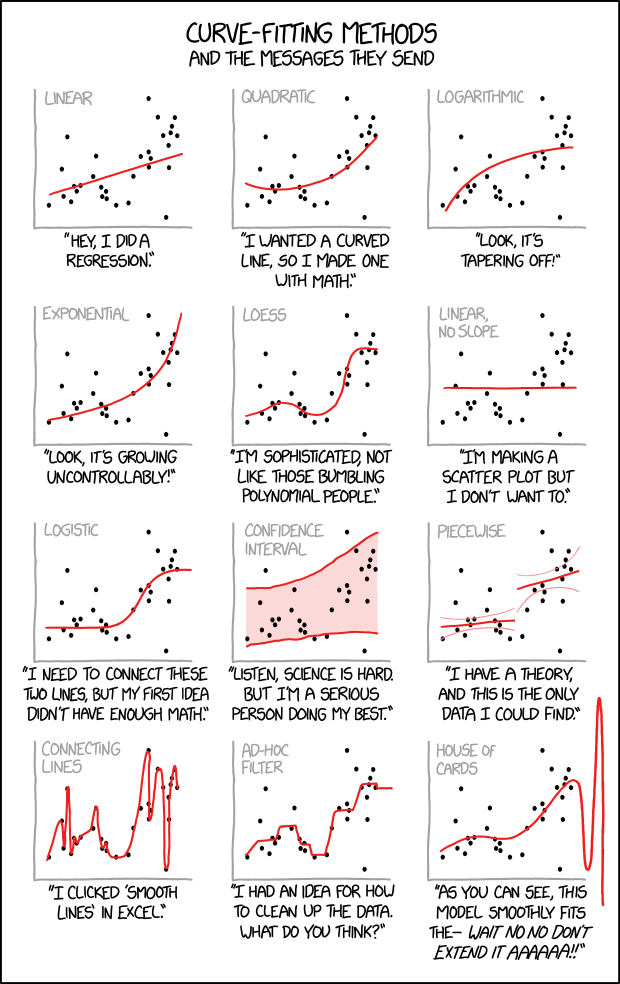
\includegraphics[height=0.55\textheight]{images/2048_curve_fitting.png}
\end{column}
\begin{column}{0.48\textwidth}
\vspace{10mm}
You have 50 features.\\[4mm]
You need 2 axes.\\[4mm]
But you also need to keep the neighborhoods intact.\\[4mm]
\highlight{How?}
\end{column}
\end{columns}
\bottomnote{XKCD \#2048 by Randall Munroe (CC BY-NC 2.5)}
\end{frame}

%=== SLIDE 3: Learning Objectives ===
\begin{frame}{What You Will Learn Today}
\begin{enumerate}
\setlength{\itemsep}{6pt}
\item Explain what t-SNE does and why it exists
\item Describe how t-SNE preserves neighborhoods (visually)
\item Recognize when t-SNE results are trustworthy vs misleading
\end{enumerate}
\bottomnote{Everything is explained with pictures, analogies, and visual diagrams --- zero formulas.}
\end{frame}

\section{The Problem}

%=== SLIDE 4: TikZ Comic C1 --- The Crowded Room ===
\begin{frame}{The Problem: Who Is Near Whom?}
\centering
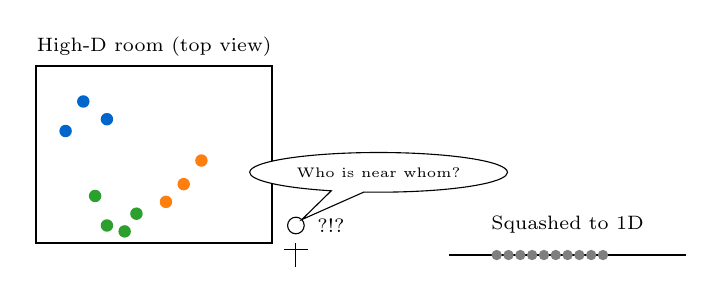
\begin{tikzpicture}[scale=0.75]
% Room rectangle
\draw[thick] (-3,0) rectangle (1,3);
\node[above] at (-1,3) {\scriptsize High-D room (top view)};
% Blue cluster
\foreach \x/\y in {-2.2/2.4, -2.5/1.9, -1.8/2.1} {\fill[mlblue] (\x,\y) circle (3pt);}
% Orange cluster
\foreach \x/\y in {-0.5/1.0, -0.2/1.4, -0.8/0.7} {\fill[mlorange] (\x,\y) circle (3pt);}
% Green cluster
\foreach \x/\y in {-1.8/0.3, -1.3/0.5, -2.0/0.8, -1.5/0.2} {\fill[mlgreen] (\x,\y) circle (3pt);}
% Stick figure at door
\draw (1.4,0.3) circle (4pt); \draw (1.4,0) -- (1.4,-0.4); \draw (1.2,-0.1) -- (1.6,-0.1);
\node[right,font=\scriptsize] at (1.6,0.3) {?!?};
\node[ellipse callout, draw, callout absolute pointer={(1.5,0.4)}, font=\tiny, fill=white] at (2.8,1.2) {Who is near whom?};
% Projected line
\draw[thick] (4,-0.2) -- (8,-0.2);
\node[above,font=\scriptsize] at (6,0) {Squashed to 1D};
\foreach \x in {4.8,5.0,5.2,5.4,5.6,5.8,6.0,6.2,6.4,6.6} {\fill[mlgray] (\x,-0.2) circle (2.5pt);}
\end{tikzpicture}

\vspace{2mm}
{\small Squashing to fewer dimensions loses the neighborhood structure.}

Dimensionality reduction must preserve which points are neighbors.
\bottomnote{t-SNE was invented specifically to solve this: preserve local neighborhoods when flattening to 2D.}
\end{frame}

%=== SLIDE 5: Why t-SNE Exists ===
\begin{frame}{What t-SNE Does (One Sentence)}
\begin{columns}[T]
\begin{column}{0.50\textwidth}
\centering
\small
\begin{tabular}{lcc}
\toprule
\textbf{Aspect} & \textbf{Linear methods} & \textbf{t-SNE} \\
\midrule
Preserves & global distances & local neighborhoods \\
Speed & fast & slow \\
Best for & preprocessing & visualization \\
\bottomrule
\end{tabular}
\end{column}
\begin{column}{0.45\textwidth}
\centering

\begin{tikzpicture}[scale=0.5]
\foreach \x/\y in {-1.5/0.3,-1.2/-0.2,-1.8/0.1,-1.0/0.5} {\fill[mlgray] (\x,\y) circle (3pt);}
\foreach \x/\y in {-1.3/-0.5,-1.6/-0.3} {\fill[mlgray] (\x,\y) circle (3pt);}
\draw[-{Stealth},thick,mlpurple] (0,0) -- (1.5,0) node[midway,above,font=\tiny] {t-SNE};
\foreach \x/\y in {3.0/0.6,3.3/0.4,2.8/0.3} {\fill[mlblue] (\x,\y) circle (3pt);}
\foreach \x/\y in {3.8/-0.4,4.1/-0.2} {\fill[mlorange] (\x,\y) circle (3pt);}
\end{tikzpicture}
\end{column}
\end{columns}

\vspace{4mm}
\highlight{t-SNE keeps nearby points nearby. That is the entire idea.}
\bottomnote{van der Maaten \& Hinton, 2008. The ``t'' is for Student's t-distribution; ``SNE'' = Stochastic Neighbor Embedding.}
\end{frame}

\section{How t-SNE Works}

%=== SLIDE 6: CHART 1 --- Swiss Roll ===
\begin{frame}{t-SNE Unrolls What Linear Methods Cannot}
\centering

\includegraphics[width=0.65\textwidth]{05b_tsne_swiss_roll/chart.pdf}
\begin{compactlist}
\item Data spirals in 3D like a rolled carpet
\item t-SNE preserves the neighborhood order along the spiral
\end{compactlist}
\bottomnote{Compare with PCA on the same data: PCA smashes the spiral flat, mixing distant points.}
\end{frame}

%=== SLIDE 7: TikZ Comic C2 --- The Spring System ===
\begin{frame}{How t-SNE Works: A Spring System}
\centering
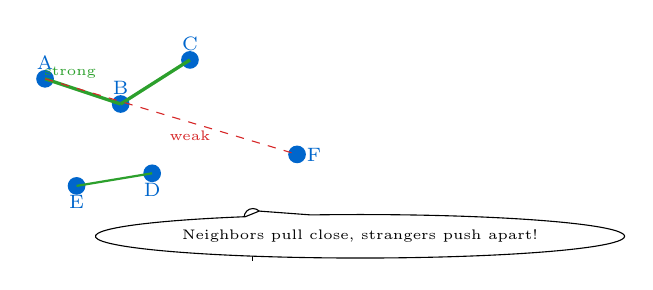
\begin{tikzpicture}[scale=0.8]
% Points
\fill[mlblue] (-1.5,1.2) circle (4pt) node[above,font=\scriptsize] {A};
\fill[mlblue] (-0.3,0.8) circle (4pt) node[above,font=\scriptsize] {B};
\fill[mlblue] (0.8,1.5) circle (4pt) node[above,font=\scriptsize] {C};
\fill[mlblue] (0.2,-0.3) circle (4pt) node[below,font=\scriptsize] {D};
\fill[mlblue] (-1.0,-0.5) circle (4pt) node[below,font=\scriptsize] {E};
\fill[mlblue] (2.5,0.0) circle (4pt) node[right,font=\scriptsize] {F};
% Strong springs (neighbors)
\draw[mlgreen,very thick] (-1.5,1.2) -- (-0.3,0.8);
\draw[mlgreen,very thick] (-0.3,0.8) -- (0.8,1.5);
\draw[mlgreen,thick] (0.2,-0.3) -- (-1.0,-0.5);
% Weak spring (strangers)
\draw[mlred,thin,dashed] (-1.5,1.2) -- (2.5,0.0);
% Labels
\node[mlgreen,font=\tiny] at (-1.1,1.3) {strong};
\node[mlred,font=\tiny] at (0.8,0.3) {weak};
% Stick figure
\draw (1.8,-1.0) circle (4pt); \draw (1.8,-1.3) -- (1.8,-1.7); \draw (1.6,-1.4) -- (2.0,-1.4);
\node[ellipse callout, draw, callout absolute pointer={(1.9,-0.9)}, font=\tiny, fill=white] at (3.5,-1.3) {Neighbors pull close, strangers push apart!};
\end{tikzpicture}

\vspace{2mm}
t-SNE connects every pair of points with a spring. Neighbors get strong springs. Strangers get weak ones.
\bottomnote{The ``springs'' are probability-based: high probability = strong pull, low probability = weak push.}
\end{frame}

%=== SLIDE 8: CHART 2 --- Cluster Separation ===
\begin{frame}{The Payoff: Clean Cluster Separation}
\centering

\includegraphics[width=0.60\textwidth]{06c_tsne_cluster_projection/chart.pdf}
\begin{compactlist}
\item Each color is a different group in the original high-D data
\item t-SNE pulls clusters apart so you can see them
\item Warning: distances BETWEEN clusters are not meaningful
\end{compactlist}
\bottomnote{t-SNE excels at revealing IF clusters exist. It does NOT tell you how far apart they are.}
\end{frame}

%=== SLIDE 9: Visual Formulas VF1 + VF2 --- Two Lenses ===
\begin{frame}{Two Different Lenses for Measuring Similarity}
\begin{columns}[T]
\begin{column}{0.47\textwidth}
\centering
{\small\textbf{In High-D: Gaussian Lens}}

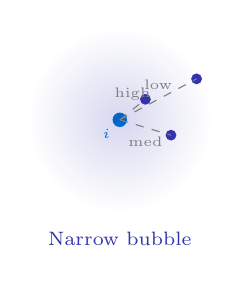
\begin{tikzpicture}[scale=0.65]
\shade[inner color=mlpurple!20, outer color=white] (0,0) circle (1.8);
\fill[mlblue] (0,0) circle (4pt) node[below left,font=\tiny] {$i$};
\fill[mlpurple] (0.5,0.4) circle (3pt);
\fill[mlpurple] (1.0,-0.3) circle (3pt);
\fill[mlpurple] (1.5,0.8) circle (3pt);
\draw[dashed,mlgray] (0,0) -- (0.5,0.4) node[midway,above,font=\tiny] {high};
\draw[dashed,mlgray] (0,0) -- (1.0,-0.3) node[midway,below,font=\tiny] {med};
\draw[dashed,mlgray] (0,0) -- (1.5,0.8) node[midway,above,font=\tiny] {low};
\node[below,font=\scriptsize,mlpurple] at (0,-2.0) {Narrow bubble};
\end{tikzpicture}
\end{column}
\begin{column}{0.47\textwidth}
\centering
{\small\textbf{In 2D: Student-t Lens}}

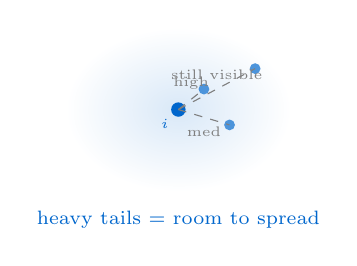
\begin{tikzpicture}[scale=0.65]
\shade[inner color=mlblue!15, outer color=white] (0,0) ellipse (2.2 and 1.6);
\fill[mlblue] (0,0) circle (4pt) node[below left,font=\tiny] {$i$};
\fill[mlblue!70] (0.5,0.4) circle (3pt);
\fill[mlblue!70] (1.0,-0.3) circle (3pt);
\fill[mlblue!70] (1.5,0.8) circle (3pt);
\draw[dashed,mlgray] (0,0) -- (0.5,0.4) node[midway,above,font=\tiny] {high};
\draw[dashed,mlgray] (0,0) -- (1.0,-0.3) node[midway,below,font=\tiny] {med};
\draw[dashed,mlgray] (0,0) -- (1.5,0.8) node[midway,above,font=\tiny] {still visible};
\node[below,font=\scriptsize,mlblue] at (0,-1.8) {heavy tails = room to spread};
\end{tikzpicture}
\end{column}
\end{columns}

\vspace{2mm}
\begin{compactlist}
\item High-D uses a narrow Gaussian bubble --- only close neighbors matter
\item 2D uses a wider Student-t bubble --- far points get pushed much farther apart
\end{compactlist}
\bottomnote{The wider t-distribution lens in 2D solves the ``crowding problem'': it gives clusters room to breathe.}
\end{frame}

%=== SLIDE 10: Visual Formula VF3 --- KL Divergence ===
\begin{frame}{The Goal: Make Both Pictures Match}
\centering
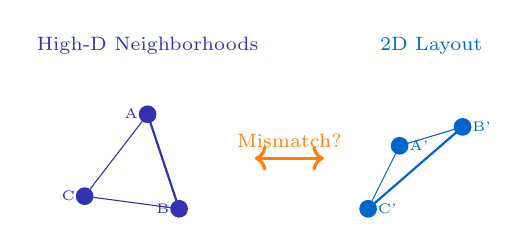
\begin{tikzpicture}[scale=0.8]
% Left group: High-D
\node[above,font=\scriptsize,mlpurple] at (-2,1.8) {High-D Neighborhoods};
\fill[mlpurple] (-2,1) circle (4pt) node[left,font=\tiny] {A};
\fill[mlpurple] (-1.5,-0.5) circle (4pt) node[left,font=\tiny] {B};
\fill[mlpurple] (-3,-0.3) circle (4pt) node[left,font=\tiny] {C};
\draw[mlpurple,thick] (-2,1) -- (-1.5,-0.5);
\draw[mlpurple] (-1.5,-0.5) -- (-3,-0.3);
\draw[mlpurple,thin] (-2,1) -- (-3,-0.3);
% Right group: 2D
\node[above,font=\scriptsize,mlblue] at (2.5,1.8) {2D Layout};
\fill[mlblue] (2,0.5) circle (4pt) node[right,font=\tiny] {A'};
\fill[mlblue] (3,0.8) circle (4pt) node[right,font=\tiny] {B'};
\fill[mlblue] (1.5,-0.5) circle (4pt) node[right,font=\tiny] {C'};
\draw[mlblue,thin] (2,0.5) -- (3,0.8);
\draw[mlblue,thick] (3,0.8) -- (1.5,-0.5);
\draw[mlblue] (2,0.5) -- (1.5,-0.5);
% Mismatch arrow
\draw[<->,very thick,mlorange] (-0.3,0.3) -- (0.8,0.3) node[midway,above,font=\scriptsize] {Mismatch?};
\end{tikzpicture}

\vspace{2mm}
\begin{compactlist}
\item Left = neighborhoods in the original data. Right = layout in 2D.
\item t-SNE moves points until the 2D layout matches the original neighborhoods as closely as possible.
\end{compactlist}
\bottomnote{Technically this is KL divergence minimization, but visually it is just ``make these two pictures agree.''}
\end{frame}

%=== SLIDE 11: Visual Formula VF4 --- Forces ===
\begin{frame}{The Engine: Attract Neighbors, Repel Strangers}
\centering
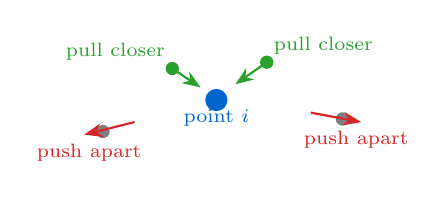
\begin{tikzpicture}[scale=0.8]
% Center point
\fill[mlblue] (0,0) circle (5pt) node[below,font=\scriptsize] {point $i$};
% Nearby points with green pull arrows
\fill[mlgreen] (0.8,0.6) circle (3pt);
\draw[-{Stealth},mlgreen,thick] (0.8,0.6) -- (0.3,0.25) node[above right,font=\scriptsize,pos=0.1] {pull closer};
\fill[mlgreen] (-0.7,0.5) circle (3pt);
\draw[-{Stealth},mlgreen,thick] (-0.7,0.5) -- (-0.25,0.2) node[above left,font=\scriptsize,pos=0.1] {pull closer};
% Distant points with red push arrows
\fill[mlgray] (2.0,-0.3) circle (3pt);
\draw[-{Stealth},mlred,thick] (1.5,-0.2) -- (2.3,-0.35) node[below,font=\scriptsize,pos=0.9] {push apart};
\fill[mlgray] (-1.8,-0.5) circle (3pt);
\draw[-{Stealth},mlred,thick] (-1.3,-0.35) -- (-2.1,-0.55) node[below,font=\scriptsize,pos=0.9] {push apart};
\end{tikzpicture}

\vspace{2mm}
\begin{compactlist}
\item Green arrows: neighbors that are too far apart get pulled closer
\item Red arrows: non-neighbors that are too close get pushed apart
\item Every point feels these forces from every other point, every iteration
\end{compactlist}
\bottomnote{This is gradient descent in disguise: the forces ARE the gradient. Hundreds of iterations until equilibrium.}
\end{frame}

\section{Going Deeper}

%=== SLIDE 12: VF5 + CHART 3 --- Perplexity ===
\begin{frame}{The One Knob You Must Tune: Perplexity}
\begin{columns}[T]
\begin{column}{0.45\textwidth}
\centering
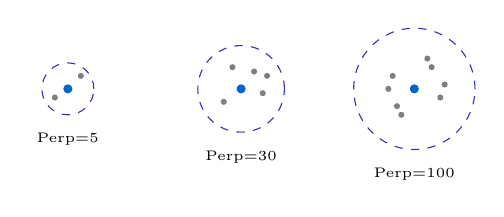
\begin{tikzpicture}[scale=0.55]
% Perp=5
\draw[dashed,mlpurple] (-4,0) circle (0.6);
\fill[mlblue] (-4,0) circle (3pt);
\fill[mlgray] (-3.7,0.3) circle (2pt); \fill[mlgray] (-4.3,-0.2) circle (2pt);
\node[below,font=\tiny] at (-4,-0.8) {Perp=5};
% Perp=30
\draw[dashed,mlpurple] (0,0) circle (1.0);
\fill[mlblue] (0,0) circle (3pt);
\foreach \x/\y in {0.3/0.4,-0.4/-0.3,0.5/-0.1,-0.2/0.5,0.6/0.3} {\fill[mlgray] (\x,\y) circle (2pt);}
\node[below,font=\tiny] at (0,-1.2) {Perp=30};
% Perp=100
\draw[dashed,mlpurple] (4,0) circle (1.4);
\fill[mlblue] (4,0) circle (3pt);
\foreach \x/\y in {4.4/0.5,3.6/-0.4,4.6/-0.2,3.5/0.3,4.3/0.7,3.7/-0.6,4.7/0.1,3.4/0.0} {\fill[mlgray] (\x,\y) circle (2pt);}
\node[below,font=\tiny] at (4,-1.6) {Perp=100};
\end{tikzpicture}
\end{column}
\begin{column}{0.50\textwidth}
\centering

\includegraphics[width=\textwidth]{top10_20_tsne_perplexity_grid/chart.pdf}
\end{column}
\end{columns}

\vspace{1mm}
\begin{compactlist}
\item Perplexity controls how many neighbors each point considers. Always try multiple values.
\end{compactlist}
\bottomnote{Default perplexity = 30 in sklearn. Try 5, 30, and 100 to see if your clusters are robust.}
\end{frame}

%=== SLIDE 13: CHART 4 + Gotchas ===
\begin{frame}{Watch It Converge --- and Three Gotchas}
\centering

\includegraphics[width=0.55\textwidth]{top10_13_tsne_iterations/chart.pdf}

\begin{enumerate}
\setlength{\itemsep}{3pt}
\item \textcolor{mlred}{\textbf{!}} Distances between clusters mean nothing --- only within-cluster structure is real
\item \textcolor{mlred}{\textbf{!}} Different random seeds produce different layouts --- run it multiple times
\item \textcolor{mlred}{\textbf{!}} Slow on big data --- use PCA to 50 dims first, then t-SNE
\end{enumerate}
\bottomnote{If your clusters disappear when you change the random seed, they are probably not real.}
\end{frame}

\section{Application}

%=== SLIDE 14: CHART 5 + Finance ===
\begin{frame}{What t-SNE Preserves --- and Where It Shines}
\centering

\includegraphics[width=0.55\textwidth]{top10_16_tsne_distance_preservation/chart.pdf}

\begin{block}{Finance Applications}
\begin{compactlist}
\item Fraud detection: t-SNE reveals anomalous transaction clusters
\item Credit risk: visualize borrower segments in high-dimensional feature space
\item Market regimes: identify hidden market states from return data
\end{compactlist}
\end{block}
\bottomnote{t-SNE is for exploration and visualization. Never feed t-SNE coordinates into a classifier.}
\end{frame}

%=== SLIDE 15: Code Recipe ===
\begin{frame}{Try It Yourself: 4 Lines of Python}
\centering
\begin{block}{t-SNE in Python}
\ttfamily\scriptsize
from sklearn.manifold import TSNE\\
tsne = TSNE(n\_components=2, perplexity=30)\\
X\_2d = tsne.fit\_transform(X)\\
plt.scatter(X\_2d[:, 0], X\_2d[:, 1])
\end{block}

\vspace{4mm}
\highlight{That is it. Four lines. sklearn does the heavy lifting.}
\bottomnote{Always scale your data first with StandardScaler. For large datasets, reduce to 50 dims with PCA before t-SNE.}
\end{frame}

\section{Closing}

%=== SLIDE 16: TikZ Comic C3 --- The Cartographer ===
\begin{frame}{The Cartographer's Map}
\centering
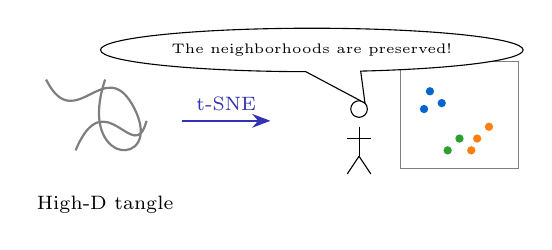
\begin{tikzpicture}[scale=0.75]
% Left: tangled scribble
\draw[mlgray,thick] (-3.5,1.5) .. controls (-3,0.5) and (-2.5,2) .. (-2,1) .. controls (-1.5,0) and (-3,0) .. (-2.5,1.5);
\draw[mlgray,thick] (-3,0.3) .. controls (-2.5,1.5) and (-2,0) .. (-1.8,0.8);
\node[below,font=\scriptsize] at (-2.5,-0.3) {High-D tangle};
% Arrow
\draw[-{Stealth},thick,mlpurple] (-1.2,0.8) -- (0.3,0.8) node[midway,above,font=\scriptsize] {t-SNE};
% Right: desk with map
\draw[mlgray] (2.5,0) rectangle (4.5,1.8);
\foreach \x/\y in {3.0/1.3,3.2/1.1,2.9/1.0} {\fill[mlblue] (\x,\y) circle (2pt);}
\foreach \x/\y in {3.8/0.5,4.0/0.7,3.7/0.3} {\fill[mlorange] (\x,\y) circle (2pt);}
\foreach \x/\y in {3.3/0.3,3.5/0.5} {\fill[mlgreen] (\x,\y) circle (2pt);}
% Stick figure at desk
\draw (1.8,1.0) circle (4pt); \draw (1.8,0.7) -- (1.8,0.2); \draw (1.6,0.5) -- (2.0,0.5);
\draw (1.8,0.2) -- (1.6,-0.1); \draw (1.8,0.2) -- (2.0,-0.1);
\node[ellipse callout, draw, callout absolute pointer={(1.9,1.1)}, font=\tiny, fill=white] at (1.0,2.0) {The neighborhoods are preserved!};
\end{tikzpicture}

\vspace{2mm}
t-SNE turns high-dimensional tangles into readable maps --- if you tune it right.
\bottomnote{t-SNE: your best tool for seeing if clusters exist in high-dimensional data.}
\end{frame}

%=== SLIDE 17: Key Takeaways ===
\begin{frame}{Three Things to Remember}
\begin{enumerate}
\setlength{\itemsep}{6pt}
\item t-SNE preserves local neighborhoods when flattening high-D data to 2D
\item It works like a spring system: neighbors attract, strangers repel
\item Always tune perplexity and run multiple seeds before trusting the layout
\end{enumerate}
\bottomnote{For preprocessing and speed, use PCA first. For visualization and cluster discovery, use t-SNE.}
\end{frame}

%=== SLIDE 18: XKCD Closing ===
\begin{frame}{Go Find the Hidden Clusters}
\centering

\includegraphics[height=0.55\textheight]{images/2400_statistics.png}
\bottomnote{XKCD \#2400 by Randall Munroe (CC BY-NC 2.5). Next: try the Jupyter notebook with real financial data!}
\end{frame}

\end{document}
